\begin{figure*}
\pgfplotsset{
 minor tick num=3,
 small,
 every axis/.style={thick,width=0.55\textwidth,height=0.20\textwidth},
 legend pos = north east,
 axis on top,
 normalise/.style 2 args={
  scaled x ticks=manual:{}{% 
   \pgfmathparse{ ( ##1 - (#1) ) }%
  }
 }
}
\begin{tabular}{cc}
$z=\SI{10}{\micro\meter}$ & $z=\SI{10}{\micro\meter}$ \\
\begin{tikzpicture}[baseline,trim axis left]
 \begin{axis}[restrict x to domain=31:100,normalise={30}{30}]
\addplot[color=Dark23qual1] file {wiggles/data/2-norm.dat};
\addplot[color=Dark23qual1,mark=o,mark size={1.500},only marks,mark repeat=3]
file {wiggles/data/near02-line-mod-norm.txt};
%\addlegendentry{$z=\SI{10}{\micro\meter}$}
\node[anchor=base east] at (0.430\textwidth,-0.009\textwidth)
{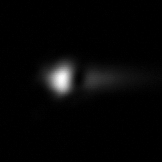
\includegraphics[height=0.11\textwidth,keepaspectratio]{wiggles/images/bw/123-11.png}};
%\addplot graphics [xmin=60,xmax=80,ymin=-0.01,ymax=0.4] {wiggles/images/bw/321-1.png};
\end{axis}
\end{tikzpicture}%
&
\begin{tikzpicture}[baseline,trim axis right]
 \begin{axis}[restrict x to domain=-9:60,normalise={-10}{-10}]
\addplot[color=Dark23qual1] file {wiggles/data/2b-norm.dat};
\addplot[color=Dark23qual1,mark=o,mark size={1.50},only marks,mark repeat=3]
file {wiggles/data/conenear-line-mod-norm.txt};
\node[anchor=base east] at (0.430\textwidth,-0.009\textwidth)
{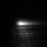
\includegraphics[height=0.11\textwidth,keepaspectratio]{wiggles/images/bw/conenear.png}};
%\addlegendentry{$z=\SI{10}{\micro\meter}$}
\end{axis}
\end{tikzpicture}%
\\
$z=\SI{1.0}{\milli\meter}$ & $z=\SI{1.0}{\milli\meter}$ \\
\begin{tikzpicture}[baseline,trim axis left]
 \begin{axis}[restrict x to domain=475:725,normalise={500}{}]
\addplot[color=Dark23qual2] file {wiggles/data/3-norm.dat};
\addplot[color=Dark23qual2,mark=o,mark size={1.50},only marks,mark repeat=3]
file {wiggles/data/midfield-line-mod-norm.txt};
\node[anchor=base east] at (0.430\textwidth,-0.009\textwidth)
{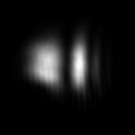
\includegraphics[height=0.11\textwidth,keepaspectratio]{wiggles/images/bw/midfield.png}};
\end{axis}
\end{tikzpicture}%
&
\begin{tikzpicture}[baseline,trim axis right]
\begin{axis}[restrict x to domain=1100:1350,normalise={1100}{}]
\addplot[color=Dark23qual2] file {wiggles/data/3b1-norm.dat};
\addplot[color=Dark23qual2,mark=o,mark size={1.50},only marks,mark repeat=3]
file {wiggles/data/conemid03-line-mod-norm.txt};
\node[anchor=base east] at (0.430\textwidth,-0.009\textwidth)
{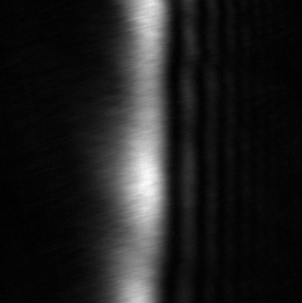
\includegraphics[height=0.11\textwidth,keepaspectratio]{wiggles/images/bw/321-7.png}};
%\addlegendentry{$z=\SI{0.1}{\milli\meter}$}
\end{axis}
\end{tikzpicture}%
\\
$z=\SI{100}{\milli\meter}$ & $z=\SI{100}{\milli\meter}$ \\
\begin{tikzpicture}[baseline,trim axis left]
\begin{axis}[
xlabel=detector scale,
/pgfplots/change x base,
/pgfplots/x unit=\si{\micro\meter},
restrict x to domain=54000:68000,
normalise={54000}{},
]
\addplot[color=Dark23qual3] file {wiggles/data/5-norm.dat};
\addplot[color=Dark23qual3,mark=o,mark size={1.50},only marks,mark repeat=3]
file {wiggles/data/farfield02-avg-mod-norm.txt};
%\addlegendentry{$z=\SI{100}{\milli\meter}$}
\node[anchor=base east] at (0.430\textwidth,-0.009\textwidth)
{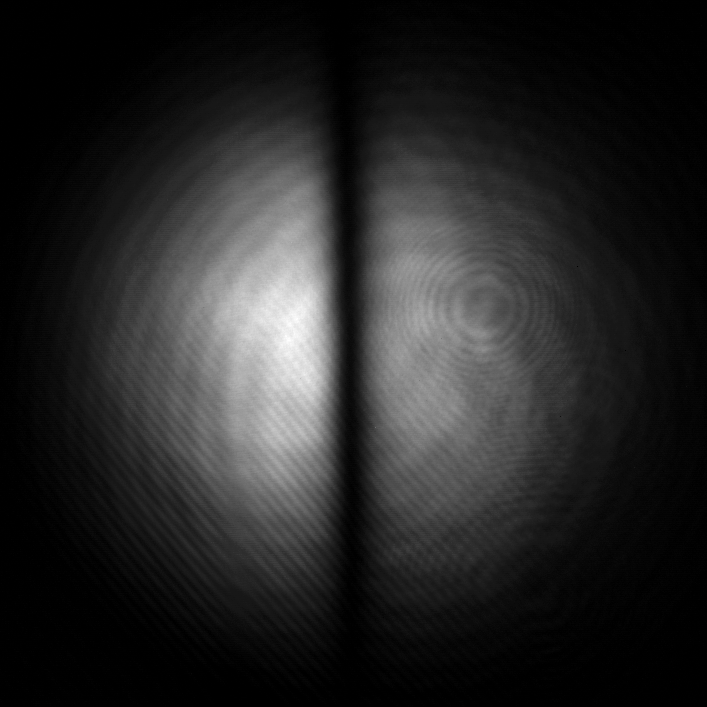
\includegraphics[height=0.11\textwidth,keepaspectratio]{wiggles/images/bw/farfield02.png}};
\end{axis}
\end{tikzpicture}%
&
\begin{tikzpicture}[baseline,trim axis right]
\begin{axis}[
xlabel=detector scale,
/pgfplots/change x base,
/pgfplots/x unit=\si{\micro\meter},
restrict x to domain=54000:68000,
normalise={54000}{},
]
\addplot[color=Dark23qual3] file {wiggles/data/5b-norm.dat};
\addplot[color=Dark23qual3,mark=o,mark size={1.50},only marks,mark repeat=3]
file {wiggles/data/farfield-cone-mod-norm.txt};
%\addlegendentry{$z=\SI{100}{\milli\meter}$}
\node[anchor=base east] at (0.430\textwidth,-0.009\textwidth)
{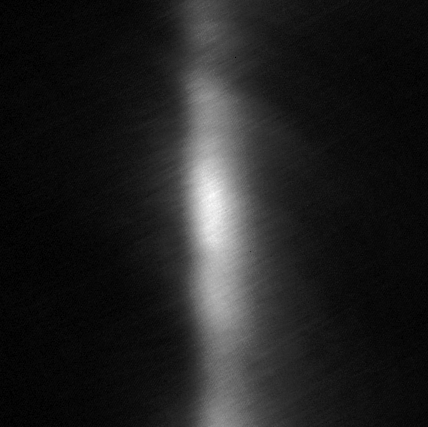
\includegraphics[height=0.11\textwidth,keepaspectratio]{wiggles/images/bw/321-9.png}};
\end{axis}
\end{tikzpicture}%
\end{tabular}
\end{figure*}
% Fresnel Numbers:
% Lorentz-Drude Model -14.48239364+1.094554854i 1.744521043e-05
% octave:24> (1.744*10^-5)^2/((0.1*10^-3)*(632.8*10^-9))
% ans =  4.8065
% octave:25> (1.744*10^-5)^2/((100*10^-3)*(632.8*10^-9))
% ans =  0.0048065
% octave:26> (1.744*10^-5)^2/((10*10^-6)*(632.8*10^-9))
% ans =  48.065
